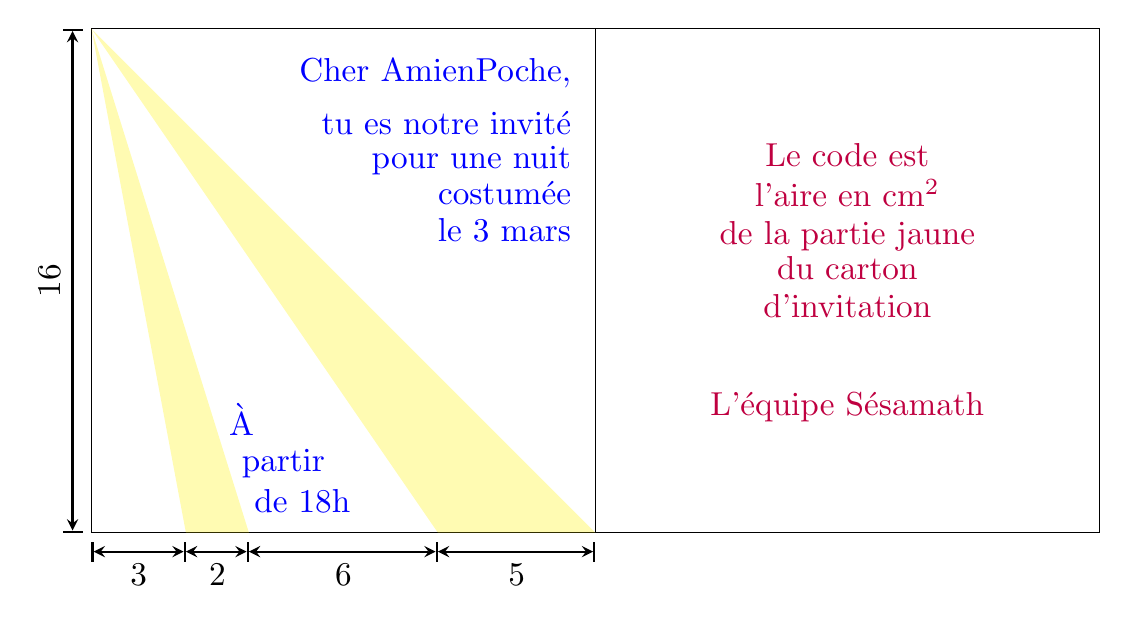
\begin{tikzpicture}[every node/.style={scale=1.2},scale=0.8]
 \draw (0,0)--(0,8)--(16,8)--(16,0)--cycle;
 \draw (8,8)--(8,0);
 \fill [yellow,opacity=0.3] (0,8)--(2.5,0)--(1.5,0)--cycle;
 \fill [yellow,opacity=0.3] (0,8)--(8,0)--(5.5,0)--cycle;
 
\draw (7.8,7.3) node[left,blue] {Cher AmienPoche,};
\draw (7.8,6.5) node[left,blue] {tu es notre invité};
\draw (7.8,5.9) node[left,blue] {pour une nuit};
\draw (7.8,5.4) node[left,blue] {costumée};
\draw (7.8,4.8) node[left,blue] {le 3 mars};

\draw (2,1.8) node[right,blue] {À};
\draw (2.2,1.1) node[right,blue] {partir};
\draw (2.4,0.5) node[right,blue] {de 18h};

\draw (12,6) node[purple] {Le code est};
\draw (12,5.4) node[purple] {l'aire en cm$^2$};
\draw (12,4.7) node[purple] {de la partie jaune};
\draw (12,4.2) node[purple] {du carton};
\draw (12,3.6) node[purple] {d'invitation};
\draw (12,2) node[purple] {L'équipe Sésamath};

\draw [thick,|<->|,>=stealth](-0.3,0)--(-0.3,8) node [midway,above,rotate=90]{16};
\draw [thick,|<->|,>=stealth](0,-0.3)--(1.5,-0.3) node [midway,below]{3};
\draw [thick,<->|,>=stealth](1.5,-0.3)--(2.5,-0.3) node [midway,below]{2};
\draw [thick,<->|,>=stealth](2.5,-0.3)--(5.5,-0.3) node [midway,below]{6};
\draw [thick,<->|,>=stealth](5.5,-0.3)--(8,-0.3) node [midway,below]{5};

\end{tikzpicture}
